\subsection{Second Experience}

\subsubsection{IPv6}
wasa

\subsubsection{Practical Exercise}

Theoretical questions:

\begin{itemize}
    \item 10.15.32.200/8: class A, NA 10.0.0.0, BA 10.255.255.255
    \item 172.20.45.7/12: class B, NA 172.16.0.0, BA 172.16.255.255
    \item 192.168.10.25/16: class C, NA 192.168.0.0, BA 192.168.255.255
\end{itemize}

After choosing the first TCP packet, we expanded and examined the IPv4 section.

\begin{figure}[htbp]
    \centering
    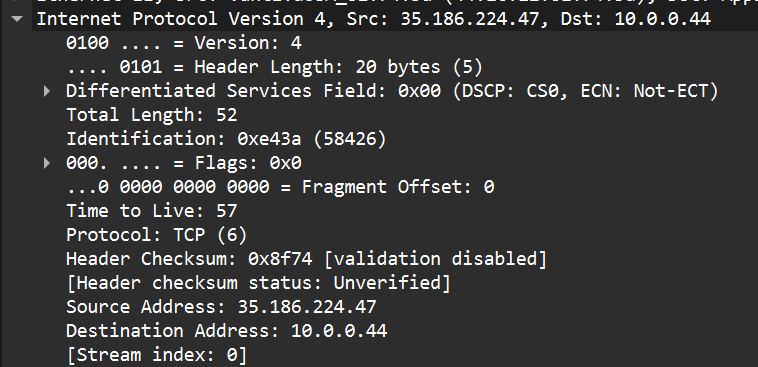
\includegraphics[width=1\linewidth]{img/2/6_1.png}
    \caption{TCP packet's IPv4 section}\label{fig:exp2_6_1}
\end{figure}

The first octet shows that both the source address \texttt{35.186.224.47} and
the destination address \texttt{10.0.04} belong to the A class.

Given that both addresses belong to the same class, and the last 3 octets are
different, we can infer a subnet mask of \texttt{255.0.0.0}.

The destination address might be a private one, as it follows the
\texttt{10.0.0.0/8} default pattern.

Finally, the TTL value of 57 might indicate that the device sending the packet
has a Linux OS.